%%
%% This is file `sample-manuscript.tex',
%% generated with the docstrip utility.
%%
%% The original source files were:
%%
%% samples.dtx  (with options: `manuscript')
%% 
%% IMPORTANT NOTICE:
%% 
%% For the copyright see the source file.
%% 
%% Any modified versions of this file must be renamed
%% with new filenames distinct from sample-manuscript.tex.
%% 
%% For distribution of the original source see the terms
%% for copying and modification in the file samples.dtx.
%% 
%% This generated file may be distributed as long as the
%% original source files, as listed above, are part of the
%% same distribution. (The sources need not necessarily be
%% in the same archive or directory.)
%%
%% Commands for TeXCount
%TC:macro \cite [option:text,text]
%TC:macro \citep [option:text,text]
%TC:macro \citet [option:text,text]
%TC:envir table 0 1
%TC:envir table* 0 1
%TC:envir tabular [ignore] word
%TC:envir displaymath 0 word
%TC:envir math 0 word
%TC:envir comment 0 0
%%
%%
%% The first command in your LaTeX source must be the \documentclass command.
%%%% Small single column format, used for CIE, CSUR, DTRAP, JACM, JDIQ, JEA, JERIC, JETC, PACMCGIT, TAAS, TACCESS, TACO, TALG, TALLIP (formerly TALIP), TCPS, TDSCI, TEAC, TECS, TELO, THRI, TIIS, TIOT, TISSEC, TIST, TKDD, TMIS, TOCE, TOCHI, TOCL, TOCS, TOCT, TODAES, TODS, TOIS, TOIT, TOMACS, TOMM (formerly TOMCCAP), TOMPECS, TOMS, TOPC, TOPLAS, TOPS, TOS, TOSEM, TOSN, TQC, TRETS, TSAS, TSC, TSLP, TWEB.
% \documentclass[acmsmall]{acmart}

%%%% Large single column format, used for IMWUT, JOCCH, PACMPL, POMACS, TAP, PACMHCI
% \documentclass[acmlarge,screen]{acmart}

%%%% Large double column format, used for TOG
% \documentclass[acmtog, authorversion]{acmart}

%%%% Generic manuscript mode, required for submission
%%%% and peer review
\documentclass[manuscript,screen,review]{acmart}
%% Fonts used in the template cannot be substituted; margin 
%% adjustments are not allowed.
%%
%% \BibTeX command to typeset BibTeX logo in the docs
\AtBeginDocument{%
  \providecommand\BibTeX{{%
    \normalfont B\kern-0.5em{\scshape i\kern-0.25em b}\kern-0.8em\TeX}}}

%% Rights management information.  This information is sent to you
%% when you complete the rights form.  These commands have SAMPLE
%% values in them; it is your responsibility as an author to replace
%% the commands and values with those provided to you when you
%% complete the rights form.
\setcopyright{acmlicensed}
\copyrightyear{2024}
\acmYear{2024}
\acmDOI{XXXXXXX.XXXXXXX}

%% These commands are for a PROCEEDINGS abstract or paper.
\acmConference[Conference acronym 'XX]{Make sure to enter the correct
  conference title from your rights confirmation email}{June 03--05,
  2018}{Woodstock, NY}
%
%  Uncomment \acmBooktitle if th title of the proceedings is different
%  from ``Proceedings of ...''!
%
\acmBooktitle{Woodstock '18: ACM Symposium on Neural Gaze Detection,
 June 03--05, 2018, Woodstock, NY} 
\acmISBN{978-1-4503-XXXX-X/18/06}


%%
%% Submission ID.
%% Use this when submitting an article to a sponsored event. You'll
%% receive a unique submission ID from the organizers
%% of the event, and this ID should be used as the parameter to this command.
%%\acmSubmissionID{123-A56-BU3}

%%
%% For managing citations, it is recommended to use bibliography
%% files in BibTeX format.
%%
%% You can then either use BibTeX with the ACM-Reference-Format style,
%% or BibLaTeX with the acmnumeric or acmauthoryear sytles, that include
%% support for advanced citation of software artefact from the
%% biblatex-software package, also separately available on CTAN.
%%
%% Look at the sample-*-biblatex.tex files for templates showcasing
%% the biblatex styles.
%%

%%
%% The majority of ACM publications use numbered citations and
%% references.  The command \citestyle{authoryear} switches to the
%% "author year" style.
%%
%% If you are preparing content for an event
%% sponsored by ACM SIGGRAPH, you must use the "author year" style of
%% citations and references.
%% Uncommenting
%% the next command will enable that style.
%%\citestyle{acmauthoryear}

%%
%% end of the preamble, start of the body of the document source.
\newcommand{\com}[1]{\textcolor{red}{\textit{#1}}}
\usepackage{lipsum}
\begin{document}

%%
%% The "title" command has an optional parameter,
%% allowing the author to define a "short title" to be used in page headers.
\title{Generalized Atomic Swaps}

%%
%% The "author" command and its associated commands are used to define
%% the authors and their affiliations.
%% Of note is the shared affiliation of the first two authors, and the
%% "authornote" and "authornotemark" commands
%% used to denote shared contribution to the research.
\author{Ras Dwivedi}
% \authornote{Both authors contributed equally to this research.}
\email{dwivedi@cse.iitk.ac.in}
% \orcid{1234-5678-9012}
\author{Sandeep Shukla}
% \authornotemark[1]
\email{sandeeps@cse.iitk.ac.in}
\affiliation{%
  \institution{Indian Institute of Technology Kanpur}
  \streetaddress{Kalyanpur, Kanpur}
  \city{Kanpur }
  \state{Uttar Pradesh}
  \country{India}
  \postcode{208016}
}

% \author{Lars Th{\o}rv{\"a}ld}
% \affiliation{%
%   \institution{The Th{\o}rv{\"a}ld Group}
%   \streetaddress{1 Th{\o}rv{\"a}ld Circle}
%   \city{Hekla}
%   \country{Iceland}}
% \email{larst@affiliation.org}

% \author{Valerie B\'eranger}
% \affiliation{%
%   \institution{Inria Paris-Rocquencourt}
%   \city{Rocquencourt}
%   \country{France}
% }

% \author{Aparna Patel}
% \affiliation{%
%  \institution{Rajiv Gandhi University}
%  \streetaddress{Rono-Hills}
%  \city{Doimukh}
%  \state{Arunachal Pradesh}
%  \country{India}}

% \author{Huifen Chan}
% \affiliation{%
%   \institution{Tsinghua University}
%   \streetaddress{30 Shuangqing Rd}
%   \city{Haidian Qu}
%   \state{Beijing Shi}
%   \country{China}}

% \author{Charles Palmer}
% \affiliation{%
%   \institution{Palmer Research Laboratories}
%   \streetaddress{8600 Datapoint Drive}
%   \city{San Antonio}
%   \state{Texas}
%   \country{USA}
%   \postcode{78229}}
% \email{cpalmer@prl.com}

% \author{John Smith}
% \affiliation{%
%   \institution{The Th{\o}rv{\"a}ld Group}
%   \streetaddress{1 Th{\o}rv{\"a}ld Circle}
%   \city{Hekla}
%   \country{Iceland}}
% \email{jsmith@affiliation.org}

% \author{Julius P. Kumquat}
% \affiliation{%
%   \institution{The Kumquat Consortium}
%   \city{New York}
%   \country{USA}}
% \email{jpkumquat@consortium.net}

%%
%% By default, the full list of authors will be used in the page
%% headers. Often, this list is too long, and will overlap
%% other information printed in the page headers. This command allows
%% the author to define a more concise list
%% of authors' names for this purpose.
\renewcommand{\shortauthors}{Trovato and Tobin, et al.}

%%
%% The abstract is a short summary of the work to be presented in the
%% article.
\begin{abstract}
A 2-party atomic cross-chain swap is a coordination task where two parties swap assets over two blockchains, for example, exchanging bitcoin for ether. The protocol guarantees three critical conditions: 1. Successful asset exchange occurs if both parties adhere to the protocol. 2. If any party deviates from the protocol, then no conforming party end up being worse. 3. The protocol ensures no party can leave the other in a perpetual deadlock, effectively locking their assets forever. Importantly, there is no incentive for any party to deviate from the protocol.

Hash Time Lock Contracts (\textit{HTLC}) are widely used in 2-party atomic swaps. This paper focuses on Multiparty Atomic Swaps, where assets may be collectively owned, and multiple assets may be involved in an exchange.

Our investigation reveals that the 2-party \textit{HTLC} framework breaks down when applied to multiparty swaps. Subsequently, we introduce a modified \textit{HTLC} protocol tailored for multiparty swaps, which requires $O(n)$ messages for an $n$-party swap. This new protocol addresses the complexities of multiparty exchanges, offering an efficient and secure solution for exchanging assets involving multiple parties. When reduced to 2-party, our protocol conducts atomic swaps without timelocks with similar message complexity as \textit{HTLC}.
    
    % In this paper,, we investigate the general form of HTLC. 
    % HTLC is a commonly used protocol for the atomic swap, which locks the assets for a time period.  
    % In this paper we present novel protocol to conduct atomic swaps without time locking. We further generalize the notion of the swap involving multiple party over the two ledger. While Hash-Time lock contracts are not sufficient in generealized case, we present a modified hash time lock contract that can handle byzantine adversary.


\end{abstract}

%%
%% The code below is generated by the tool at http://dl.acm.org/ccs.cfm.
%% Please copy and paste the code instead of the example below.
%%
\begin{CCSXML}
<ccs2012>
 <concept>
  <concept_id>00000000.0000000.0000000</concept_id>
  <concept_desc>Do Not Use This Code, Generate the Correct Terms for Your Paper</concept_desc>
  <concept_significance>500</concept_significance>
 </concept>
 <concept>
  <concept_id>00000000.00000000.00000000</concept_id>
  <concept_desc>Do Not Use This Code, Generate the Correct Terms for Your Paper</concept_desc>
  <concept_significance>300</concept_significance>
 </concept>
 <concept>
  <concept_id>00000000.00000000.00000000</concept_id>
  <concept_desc>Do Not Use This Code, Generate the Correct Terms for Your Paper</concept_desc>
  <concept_significance>100</concept_significance>
 </concept>
 <concept>
  <concept_id>00000000.00000000.00000000</concept_id>
  <concept_desc>Do Not Use This Code, Generate the Correct Terms for Your Paper</concept_desc>
  <concept_significance>100</concept_significance>
 </concept>
</ccs2012>
\end{CCSXML}

\ccsdesc[500]{Do Not Use This Code~Generate the Correct Terms for Your Paper}
\ccsdesc[300]{Do Not Use This Code~Generate the Correct Terms for Your Paper}
\ccsdesc{Do Not Use This Code~Generate the Correct Terms for Your Paper}
\ccsdesc[100]{Do Not Use This Code~Generate the Correct Terms for Your Paper}

%%
%% Keywords. The author(s) should pick words that accurately describe
%% the work being presented. Separate the keywords with commas.
\keywords{Do, Not, Us, This, Code, Put, the, Correct, Terms, for,
  Your, Paper}

%% A "teaser" image appears between the author and affiliation
%% information and the body of the document, and typically spans the
%% page.
%\begin{teaserfigure}
%  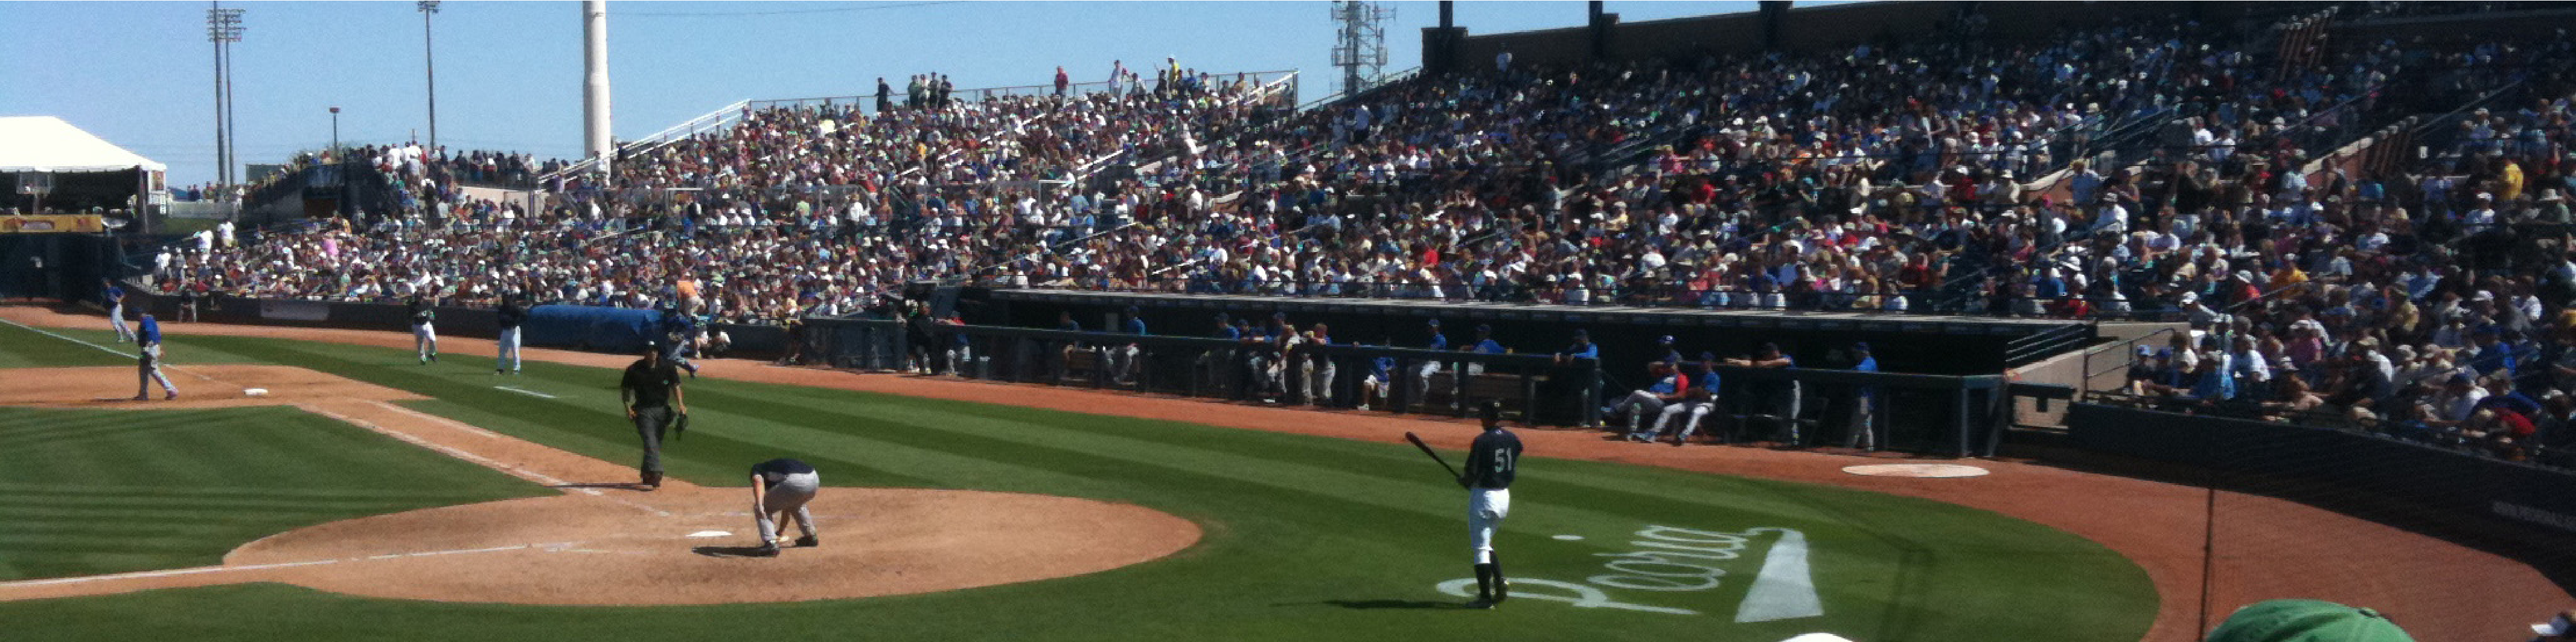
\includegraphics[width=\textwidth]{sampleteaser}
%  \caption{Seattle Mariners at Spring Training, 2010.}
%  \Description{Enjoying the baseball game from the third-base
%  seats. Ichiro Suzuki preparing to bat.}
%  \label{fig:teaser}
%\end{teaserfigure}

\received{20 February 2007}
\received[revised]{12 March 2009}
\received[accepted]{5 June 2009}

%%
%% This command processes the author and affiliation and title
%% information and builds the first part of the formatted document.
\maketitle

\section{Introduction}
\textcolor{violet}{The aim of this section is to explain atomic swaps}

The advent of Bitcoin in 2009 marked a significant milestone in the realm of digital currency, revolutionizing financial transactions globally. Subsequently, a multitude of Distributed Ledger Technologies (DLTs) emerged, each with its unique features. Interoperability between these diverse ledgers became a paramount requirement, and one of the instrumental approaches to achieving this is through the implementation of atomic swaps.

In essence, an atomic swap serves as a protocol facilitating the seamless exchange of assets between two parties operating on distinct blockchains. At its core, a "fair" atomic swap protocol is designed to eliminate any incentives for either party to deviate from the established protocol. Crucially, if one party does deviate, the other party does not suffer any disadvantage. This guarantees that the outcome of the exchange is either successful, with both parties obtaining the desired assets, or unsuccessful, with both retaining their original assets.

Importantly, an atomic swap ensures that, at no point, does one party gain control over both assets. This inherent characteristic enhances the security and trustworthiness of the exchange process. Additionally, the protocol prevents the creation of a deadlock situation where assets are perpetually locked, ensuring a smooth and reliable execution of the swap.



\com{What is the fair part in the protocol}
\section{Motivation}
\textbf{ Here there should be some data about the HTLC contracts and the swaps}
\com { Here should be a description of both version of atomic swaps}
A number of blockchain and there by crypto currencies have been introduced since the bitcoin. Due to the sheer number of the blockchains and the cryptocurrency, it becomes necessary to make them interoperable. One of the ways to make the blockchains interoperable is through the relay chain, with the contract written in the mainchain. Cosmos hub and other operates in this fashion. This is workable because all the relay chain communicate to the mainchain and the mainchain has the way to know the status of the relay chain. \\
But in case of the hetrogenous blockchain it is not possible. heterogenous blockchain have no way of communicating with each other and no way to verify the status of the contract or the account in other blockchain, except may be through some oracle. But then these oracle because external source of truth, which may be compromised. \\
Atomic swap is the third way to make the blockchain interoperable. This method is typically used for the exchange of the token or the coin among the parties that have account on both the blockchain. Idea, is that eithere the swap should happen, or nothing should happen. One party should  not have any advantage over the other party. This party should not be able to gain control over both the asset, not it should be able to forcee the other party into  a deadlock situation thereby locking the funds. 
\com{ use only of the following : token, funds or the coins}\\
HTLC \cite{} is the most common way to create the atomic swap. Unfortunately, HTLC is limited to only two parties. But in general the swap may not be limited to two parties. For example we might have the generic situation where in Ledger $\mathcal{L}_1$ two parties $A$ and $B$ might both want to exchange the asset $\alpha$ and $\beta$ with $C$ on ledger $\mathcal{L}_2$ for the joint ownership of the asset $\gamma$. Now, if both $A$ and $B$ trust each other, the traditional HTLC is possible,  However if $A$ and $B$ are also distrusting party, then we show that the traditional HTLC fails. To overcome this problem we present a general version of the HTLC. \\

\textbf{Organization of paper:} In this paper we fist show the scenario where the conventional HTLC fails. We then present a two-party HTLC protocol, which does not need any time locking. Building on this idea we presnet a generic n-party HTLC protocol. 
\section{Background work}
\com{Here should be the protocols for the background work}
\begin{itemize}
	\item Working of HTLC
	In two party $HTLC$ both the parties Alice, $A$ and Bob $B$ has thee account on ledger $\mathcal{L}_1$ and $\mathcal{L}_2$. Alice wants to asset $\alpha$ on $\mathcal{L}_1$ for the asset $\beta$ on $\mathcal{L}_2$. \\
	To faciliate the exchange, Alice creates a smart contract $\mathbb{S}_1$ and locks the asset $\alpha$. With secret $s$ and for the $\mathcal{N}$ blocks. Bob then verifies the contract on Ledger $\mathcal{L}_1$ and deploys the contract $\mathbb{S}_2$ on $\mathcal{L}_2$ which locks the Bob's asset $\beta$. Bob uses the same the secret hash to lock his asset, but his asset is locked for the lesser period of time, say $N-\delta$ block. 
	When Alice sees the Bob's smart contract, she then unlocks the Bob's contract $\mathbb{S}_2$and takes posession of the asset $\beta$ on $\mathcal{L}_2$. Bob now knows the secret $s$ and can unlock the Alice's smart contract $\mathbb{s}_1$  and takes the asset $\alpha$. Here the time difference between the locks $\delta$ should be sufficient enough to Bob the confidence to claim asset $\alpha$ before the lock expires and the asset can be claimed again by Alice. Also, we assume that the transaction prepared are includded in the block, such that there is no denial of the service attack. Otherwise Bob can know the secret $s$ from the dropped transaction and claim Alice asset $\alpha$ without forfeiting his asset $\beta$ \\
	
	It is worth noting that \textit{HTLC} protocol requires that time locking in present at both the blockchain. Blockchain such as Moreo \cite{} does not have scripting language rich enough to create the time locks. It was shown by \cite{} that time locking is not required at both the ends, and with the use of adaptive signatures \cite{} one can conduct atomic swaps with the time locking at only one of the blockchain. 
	
%	But these protocols are restricted to the two-party atomic swap protocol. We are interested in more general case which we describe below. Let $ \mathcal{A} = {A1, A_2, ... A_m}$ be the parties interested in the atomic swap with $\mathcal{B}=B_1, B_2 ... B_n$ where $\mathcal{A}$ and $\mathcal{B}$ might not be mutually exclusive. Assets to be swapped are $\Alpha = {\alpha_1, \alpha_2, .... \alpha_m}$ be assets to be swappedd in ledger $\mathcal{L}_1$ and $\Beta = { \beta_1, \beta_2, ... \beta_m} $ be the assets that are to be swapped in ledger $\mathcal{L}_2$. Let $I_{ij}$ \\
\com{Explain the need for the multiparty swap}
	\begin{itemize}
		\item Joint Ownership of assets
		\item Portfolio rebalancing
		\item Assembly line ? car parts + plus cash for car 
	\end{itemize}
	But these protocols are restricted to the two-party atomic swap protocol. We are interested in more general case which we describe below. Ledger $\mathcal{L}_1$ contains assets $ \mathbb{A}= \{\alpha_1, \alpha_2, ....., \alpha_m \}$ and ledger $\mathcal{L}_2$ contains assets $\mathbb{B} = \{\beta_1, \beta_2, ....., \beta_n \}$ which are to be swapped. Let the swap contains $p$ parties. Boolean $I_{\alpha}^{ij}$ is \textbf{True} if party $j$ was the initial owner of the asset $\alpha_i$, \textbf{False} otherwise. Similarly $I_{\beta}^{ij}$ is \textbf{True} if party $j$ was the initial owner of the asset $\beta_i$, \textbf{False} otherwise. Boolean $O_{\alpha}^{ij}$ is \textbf{True} if party $j$ is the final owner of the asset $\alpha_i$, \textbf{False} otherwise. Similarly $O_{\beta}^{ij}$ is \textbf{True} if party $j$ is the final owner of the asset $\beta_i$, \textbf{False} otherwise. 
	
	\com{Define the atomic swap}
	A two party atomic swap is defined as follows.
	Let $P$ and $Q$ be the two parties. $P$ owns the asset $i_P$ and $Q$ owns the asset $I_Q$. The swap is consider successful if at the end of the protocol $P$ possesses $I_Q$ and $Q$ possess $I_P$. The protocol is considered \textbf{fair} if either the swap completes or nothing happens at all
	
	A multiparty atomic swap is defined as follows. Let there be $m+n$ assets. Assets are owned by parties $\{j \}$ such that $I_{\alpha}^{ij=1}$. At the end of the swap, the owners of the asset $\alpha_i$ should be $O_{alpha}^{ij}$
	

	\item working of Generic swap by IBM guys
	\item swapping protocol by Ras, Tushar and Sandeep
\end{itemize}
\section{Why two party HTLC does not work}
Suppose a simple case of three party swap. Parties $A$ and $B$ owns asset $\alpha$ on ledger $\mathcal{L}_1$ and $C$ owns the asset $\gamma$ on ledger $\mathcal{L}_2$. $A$ and $B$ wants to exchange the joint ownership of $\alpha$ for the join ownership of $\gamma$, and $C$ wants to swap $\gamma$ for $\alpha$
Suppose $A$ and $B$ generates a shared secret and use that to create the smart contract $\mathbb{S}_1$ and locks their asset $\alpha$. Now, if we assume that $B$ is malicious he may collude with $C$ and share the secret with $C$. $C$ in turn uses the secret to unlock the contract and claim $\alpha$ without even locking his asset $\gamma$. So, a single shared secret, does not work in case of shared asset.\\
How about if we have two secret instead of one. Let us assume that $A$ and $B$ modifies the 2-party \textit{HTLC} and locks $\alpha$ with secrets $s_A$ and $s_B$. For $C$ to claim $\alpha$ he must know both $s_A$ and $s_B$. Assuming that at least one of $A$ and $B$ is honest, $C$ cannot claim $\alpha$ without actually knowing the secrets. So, he deploys the \textit{HTLC} contract locking the assets with the hash of $s_A$ and $s_B$. Without loss of generality, assume $B$ is malicious and has colluded with $C$. Now, $B$ waits for $A$ to first unlock the $C$'s smart contract. if $A$ does not unlocks first, then $B$ simply waits for the time lock to expire and thus not allowing the exchange to happen. In case $A$ reveals the secret $s_A$ first, $B$ still does not unlock the $C$'s smart contract, enabling $C$ to reclaim his asset after the time lock expires. But $B$ shares his secret $s_B$ privately with $C$ which allows $C$ to claim $\alpha$ without giving $\gamma$. 
Thus a 2-party \textit{HTLC} does not work in the multiparty case.

\cite{ibm} modified the HTLC contract using MPC. Here the secret is revealed simultaneously using MPC. This may result in significant cryptographic computational overhead. 
\com{A Table to compare the algorithm, in terms of message and storage complexity}


\section{A time lock free HTLC protocol}
In this section we describe an optimized version of the time lock free protocol by \cite{}. In their protocol party $A$ owns $\alpha$ and $B$ owns $\beta$ and they wants to swap their assets
The protocol works in 5 stages.
\com{refined or optimized}
\begin{enumerate}
	\item\textbf{ exchange of hashes:}  $A$ and $B$ both generates the secrets $s_A, r_A$ and $s_B, r_B$ and exchanges the hashes of the secret over the private channel
	\item \textbf{deployment of the contract:} Both $A$ and $B$ deploys the contract. $A$'s contract concerns the asset $\alpha$ and requires secrets $s_A$ and $s_B$ for successful transfer. It requires $r_A$ to quit the contract and $r_A, r_B$ to abort the contract. Quitting happens if $B$ has not commited for the exchange, and anort happens if $B$ has quit his contract after committing. 
	\com {rephrase is needed}
	\item \textbf{Freeze:} $B$ can freeze $A$'s contract by passing secret $s_B$ in to $A$'s contract on $\mathcal{L}_1$ . If $B$ freezes $A$'s contract, then $A$ cannot quit. Similary $A$ can freeze $B$'s contract by passing $s_A$ to $B$'s contract on $\mathcal{L}_2$. 
	\item \textbf{exchange of asset :} Once $A$ knows about $s_B$, he can then pass $s_B$ to the $B$'s contract on $\mathcal{L}_2$.  and claim $\beta$, Similart $B$ can pass $s_A$ to $A$'s contract and claim $\alpha$
	\item \textbf{quit and abort :} In case $B$ does not deploy his contract, $A$ can use $r_A$ on his smart contract on $\mathcal{L}_1$ and quit the swap. $A$ can only quit if his contract is not frozen. If frozen by $B$, $A$ should claim $B$. But in case $B$ freezes $A$'s contract, and quits his own, he would have to reveal $r_B$. by passing $r_B$ to his contract, $A$ can abort the swap. Knowing $r_B$ shows that $B$ has quit and hence $A$ should also quit. \\
	\com{rephrase}
	\com{comment on the optimization}\\
	\com{Diagram is needed}
	The original version of the protocol included two more secrets, each by $A$ and $B$, which was used to freeze the contract. We optimzed the secret by removing the redundant variables.

	
\end{enumerate}
	We noted that this protocol also suffers from the same vulnerability in case of multi party swap. for example. Let $A$ and $B$ jointly owns $\alpha$ and $C$ owns $\gamma$ and they want to swap the assets. 	
	\begin{itemize}
		\item In case of shared secret between $A$ and $B$, $B$ can collude with $C$ allowing $C$ to quit his swap while claiming $\alpha$. It is worth noting that even when $C$ tries to claim $\alpha$ he has to reveal his own secrets. and if honest $A$ is quick enough, he can stop the unfair execution, by aborting as soon as $C$ quits. In case $C$ freezes the asset, then claiming $\beta$ before $C$ can quit. But, due to the network latency and congestion $C$ has a fair chance to claim $\alpha$ while retaining $\gamma$
		\item In case $A$ and $B$ uses their individual secrets, the problem still persists like in the previous case. 
		It has to be notes the $B$'s contract can only be frozen if both $s_A$ and $s_B$ is available. if this is not the case, and contract is frozen as soon as $A$ frozes $C$'s contract, then $B$ can choose not to reveal either of the secret and create a deadlock for $C$ as $C$ would not be able to claim $\alpha$ without knowing $s_B$ and she cannot abort without knowing $r_B$, both of which are controlled by $B$.
	\end{itemize}

\section{A generalized HTLC protocol}
In this section we present a generalized HTLC protocol. Our protocol does not use MPC to generate a shared secret. 
In this section we present a generalized atomic swap between $A$, $B$ jointly owning $\alpha$ and $C$ and $D$ jointly owning $\beta$\\
\com{Explain who deploys the contract, and how is the asset locked. The best way is to transfer the asset first to the smart contract, and then apply the locking mechanism}\\
\com{unlike freeze, which is \textit{AND} function, the quit and abort has to be \textit{OR} funciton}
\begin{itemize}
	\item Exchange of hashes: Each party selects two secrets $s_i$ and $r_i$ and calculates the hashes of them. These hashes are exchanged over the secure private channel
	\item Deployment of the contract: A contract is deployed on $\mathcal{L}_1$ and $\mathcal{L}_2$ blockchain. First all the parties tranfer the ownership of the asset to the smart contract, while elucidating the rules for the transfer both in case of the success of the swap or in case swap is unsuccessful and the assets are send bvack to the orginal owner. This could be best represented in form of asset to initial and final owner mappings. \\
	Contract is then locked with the hashes of the secrets of all the parites. Each sender and reciever is alloted two secret $(s_i, r_i)$, irrespective of the asset swapped. This is done to ensure that either all the swap happens at once or none of the swap happen. $s_i$ is needed to claim the asset, while $r_i$ is needed by the party $i$ to quit the protocol.
	\item Freeze: In order to freeze the asset on $\mathcal{L}_1$ all the $s_j$ from receiver of the assets should be provided. All the receiver would freeze the contract one by one. Once all the receivers secrets are available, contract would be frozen. Once frozen, the sender cannot revert back and forfeit the swap. They can although abort the swap, but that can only be done once it is proven, that the contract $\mathbb{S}_2$ on $\mathcal{L}_@$ is in Quit state. If the contract $\mathbb{S}_2$  is Quit, then all the receivers secret $r_j$ is available and hence they can be used to prove that the receiving party has quit thee swap
	\item Resolve: Resove protocol involves claiming of the asset. If $\mathcal{A}$ wants to claim the assets of $\mathcal{B}$ then each $p_i$ in $\mathbb{A}$ would have to invoke the resolve method of $\mathbb{S}_2$ on $\mathcal{L}_2$. Resolve method can only be invoked after freeze has been invoked on $\mathbb{S}_2$ . If the party $p_i \in \mathcal{B}$ wants to invoke resolve in $\mathbb{S}_1$ then they would have to invoke revoke using their own $s_{2i}$. Note that resolve and quit reveals all the $s_i$.
	
	\com{need for better wordings, and better and consistent symbols}
	
	
\end{itemize}

\section{Template Overview}
As noted in the introduction, the ``\verb|acmart|'' document class can
be used to prepare many different kinds of documentation --- a
dual-anonymous initial submission of a full-length technical paper, a
two-page SIGGRAPH Emerging Technologies abstract, a ``camera-ready''
journal article, a SIGCHI Extended Abstract, and more --- all by
selecting the appropriate {\itshape template style} and {\itshape
  template parameters}.

This document will explain the major features of the document
class. For further information, the {\itshape \LaTeX\ User's Guide} is
available from
\url{https://www.acm.org/publications/proceedings-template}.

\subsection{Template Styles}

The primary parameter given to the ``\verb|acmart|'' document class is
the {\itshape template style} which corresponds to the kind of publication
or SIG publishing the work. This parameter is enclosed in square
brackets and is a part of the {\verb|documentclass|} command:
\begin{verbatim}
  \documentclass[STYLE]{acmart}
\end{verbatim}

Journals use one of three template styles. All but three ACM journals
use the {\verb|acmsmall|} template style:
\begin{itemize}
\item {\verb|acmsmall|}: The default journal template style.
\item {\verb|acmlarge|}: Used by JOCCH and TAP.
\item {\verb|acmtog|}: Used by TOG.
\end{itemize}

The majority of conference proceedings documentation will use the {\verb|acmconf|} template style.
\begin{itemize}
\item {\verb|acmconf|}: The default proceedings template style.
\item{\verb|sigchi|}: Used for SIGCHI conference articles.
\item{\verb|sigchi-a|}: Used for SIGCHI ``Extended Abstract'' articles.
\item{\verb|sigplan|}: Used for SIGPLAN conference articles.
\end{itemize}

\subsection{Template Parameters}

In addition to specifying the {\itshape template style} to be used in
formatting your work, there are a number of {\itshape template parameters}
which modify some part of the applied template style. A complete list
of these parameters can be found in the {\itshape \LaTeX\ User's Guide.}

Frequently-used parameters, or combinations of parameters, include:
\begin{itemize}
\item {\verb|anonymous,review|}: Suitable for a ``dual-anonymous''
  conference submission. Anonymizes the work and includes line
  numbers. Use with the \verb|\acmSubmissionID| command to print the
  submission's unique ID on each page of the work.
\item{\verb|authorversion|}: Produces a version of the work suitable
  for posting by the author.
\item{\verb|screen|}: Produces colored hyperlinks.
\end{itemize}

This document uses the following string as the first command in the
source file:
\begin{verbatim}
\documentclass[sigconf,authordraft]{acmart}
\end{verbatim}

\section{Modifications}

Modifying the template --- including but not limited to: adjusting
margins, typeface sizes, line spacing, paragraph and list definitions,
and the use of the \verb|\vspace| command to manually adjust the
vertical spacing between elements of your work --- is not allowed.

{\bfseries Your document will be returned to you for revision if
  modifications are discovered.}

\section{Typefaces}

The ``\verb|acmart|'' document class requires the use of the
``Libertine'' typeface family. Your \TeX\ installation should include
this set of packages. Please do not substitute other typefaces. The
``\verb|lmodern|'' and ``\verb|ltimes|'' packages should not be used,
as they will override the built-in typeface families.

\section{Title Information}

The title of your work should use capital letters appropriately -
\url{https://capitalizemytitle.com/} has useful rules for
capitalization. Use the {\verb|title|} command to define the title of
your work. If your work has a subtitle, define it with the
{\verb|subtitle|} command.  Do not insert line breaks in your title.

If your title is lengthy, you must define a short version to be used
in the page headers, to prevent overlapping text. The \verb|title|
command has a ``short title'' parameter:
\begin{verbatim}
  \title[short title]{full title}
\end{verbatim}

\section{Authors and Affiliations}

Each author must be defined separately for accurate metadata
identification. Multiple authors may share one affiliation. Authors'
names should not be abbreviated; use full first names wherever
possible. Include authors' e-mail addresses whenever possible.

Grouping authors' names or e-mail addresses, or providing an ``e-mail
alias,'' as shown below, is not acceptable:
\begin{verbatim}
  \author{Brooke Aster, David Mehldau}
  \email{dave,judy,steve@university.edu}
  \email{firstname.lastname@phillips.org}
\end{verbatim}

The \verb|authornote| and \verb|authornotemark| commands allow a note
to apply to multiple authors --- for example, if the first two authors
of an article contributed equally to the work.

If your author list is lengthy, you must define a shortened version of
the list of authors to be used in the page headers, to prevent
overlapping text. The following command should be placed just after
the last \verb|\author{}| definition:
\begin{verbatim}
  \renewcommand{\shortauthors}{McCartney, et al.}
\end{verbatim}
Omitting this command will force the use of a concatenated list of all
of the authors' names, which may result in overlapping text in the
page headers.

The article template's documentation, available at
\url{https://www.acm.org/publications/proceedings-template}, has a
complete explanation of these commands and tips for their effective
use.

Note that authors' addresses are mandatory for journal articles.

\section{Rights Information}

Authors of any work published by ACM will need to complete a rights
form. Depending on the kind of work, and the rights management choice
made by the author, this may be copyright transfer, permission,
license, or an OA (open access) agreement.

Regardless of the rights management choice, the author will receive a
copy of the completed rights form once it has been submitted. This
form contains \LaTeX\ commands that must be copied into the source
document. When the document source is compiled, these commands and
their parameters add formatted text to several areas of the final
document:
\begin{itemize}
\item the ``ACM Reference Format'' text on the first page.
\item the ``rights management'' text on the first page.
\item the conference information in the page header(s).
\end{itemize}

Rights information is unique to the work; if you are preparing several
works for an event, make sure to use the correct set of commands with
each of the works.

The ACM Reference Format text is required for all articles over one
page in length, and is optional for one-page articles (abstracts).

\section{CCS Concepts and User-Defined Keywords}

Two elements of the ``acmart'' document class provide powerful
taxonomic tools for you to help readers find your work in an online
search.

The ACM Computing Classification System ---
\url{https://www.acm.org/publications/class-2012} --- is a set of
classifiers and concepts that describe the computing
discipline. Authors can select entries from this classification
system, via \url{https://dl.acm.org/ccs/ccs.cfm}, and generate the
commands to be included in the \LaTeX\ source.

User-defined keywords are a comma-separated list of words and phrases
of the authors' choosing, providing a more flexible way of describing
the research being presented.

CCS concepts and user-defined keywords are required for for all
articles over two pages in length, and are optional for one- and
two-page articles (or abstracts).

\section{Sectioning Commands}

Your work should use standard \LaTeX\ sectioning commands:
\verb|section|, \verb|subsection|, \verb|subsubsection|, and
\verb|paragraph|. They should be numbered; do not remove the numbering
from the commands.

Simulating a sectioning command by setting the first word or words of
a paragraph in boldface or italicized text is {\bfseries not allowed.}

\section{Tables}

The ``\verb|acmart|'' document class includes the ``\verb|booktabs|''
package --- \url{https://ctan.org/pkg/booktabs} --- for preparing
high-quality tables.

Table captions are placed {\itshape above} the table.

Because tables cannot be split across pages, the best placement for
them is typically the top of the page nearest their initial cite.  To
ensure this proper ``floating'' placement of tables, use the
environment \textbf{table} to enclose the table's contents and the
table caption.  The contents of the table itself must go in the
\textbf{tabular} environment, to be aligned properly in rows and
columns, with the desired horizontal and vertical rules.  Again,
detailed instructions on \textbf{tabular} material are found in the
\textit{\LaTeX\ User's Guide}.

Immediately following this sentence is the point at which
Table~\ref{tab:freq} is included in the input file; compare the
placement of the table here with the table in the printed output of
this document.

\begin{table}
  \caption{Frequency of Special Characters}
  \label{tab:freq}
  \begin{tabular}{ccl}
    \toprule
    Non-English or Math&Frequency&Comments\\
    \midrule
    \O & 1 in 1,000& For Swedish names\\
    $\pi$ & 1 in 5& Common in math\\
    \$ & 4 in 5 & Used in business\\
    $\Psi^2_1$ & 1 in 40,000& Unexplained usage\\
  \bottomrule
\end{tabular}
\end{table}

To set a wider table, which takes up the whole width of the page's
live area, use the environment \textbf{table*} to enclose the table's
contents and the table caption.  As with a single-column table, this
wide table will ``float'' to a location deemed more
desirable. Immediately following this sentence is the point at which
Table~\ref{tab:commands} is included in the input file; again, it is
instructive to compare the placement of the table here with the table
in the printed output of this document.

\begin{table*}
  \caption{Some Typical Commands}
  \label{tab:commands}
  \begin{tabular}{ccl}
    \toprule
    Command &A Number & Comments\\
    \midrule
    \texttt{{\char'134}author} & 100& Author \\
    \texttt{{\char'134}table}& 300 & For tables\\
    \texttt{{\char'134}table*}& 400& For wider tables\\
    \bottomrule
  \end{tabular}
\end{table*}

Always use midrule to separate table header rows from data rows, and
use it only for this purpose. This enables assistive technologies to
recognise table headers and support their users in navigating tables
more easily.

\section{Math Equations}
You may want to display math equations in three distinct styles:
inline, numbered or non-numbered display.  Each of the three are
discussed in the next sections.

\subsection{Inline (In-text) Equations}
A formula that appears in the running text is called an inline or
in-text formula.  It is produced by the \textbf{math} environment,
which can be invoked with the usual
\texttt{{\char'134}begin\,\ldots{\char'134}end} construction or with
the short form \texttt{\$\,\ldots\$}. You can use any of the symbols
and structures, from $\alpha$ to $\omega$, available in
\LaTeX~\cite{Lamport:LaTeX}; this section will simply show a few
examples of in-text equations in context. Notice how this equation:
\begin{math}
  \lim_{n\rightarrow \infty}x=0
\end{math},
set here in in-line math style, looks slightly different when
set in display style.  (See next section).

\subsection{Display Equations}
A numbered display equation---one set off by vertical space from the
text and centered horizontally---is produced by the \textbf{equation}
environment. An unnumbered display equation is produced by the
\textbf{displaymath} environment.

Again, in either environment, you can use any of the symbols and
structures available in \LaTeX\@; this section will just give a couple
of examples of display equations in context.  First, consider the
equation, shown as an inline equation above:
\begin{equation}
  \lim_{n\rightarrow \infty}x=0
\end{equation}
Notice how it is formatted somewhat differently in
the \textbf{displaymath}
environment.  Now, we'll enter an unnumbered equation:
\begin{displaymath}
  \sum_{i=0}^{\infty} x + 1
\end{displaymath}
and follow it with another numbered equation:
\begin{equation}
  \sum_{i=0}^{\infty}x_i=\int_{0}^{\pi+2} f
\end{equation}
just to demonstrate \LaTeX's able handling of numbering.

\section{Figures}

The ``\verb|figure|'' environment should be used for figures. One or
more images can be placed within a figure. If your figure contains
third-party material, you must clearly identify it as such, as shown
in the example below.
\begin{figure}[h]
  \centering
  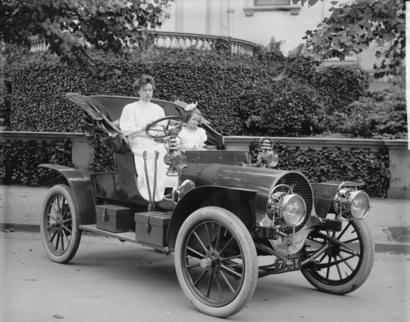
\includegraphics[width=\linewidth]{sample-franklin}
  \caption{1907 Franklin Model D roadster. Photograph by Harris \&
    Ewing, Inc. [Public domain], via Wikimedia
    Commons. (\url{https://goo.gl/VLCRBB}).}
  \Description{A woman and a girl in white dresses sit in an open car.}
\end{figure}

Your figures should contain a caption which describes the figure to
the reader.

Figure captions are placed {\itshape below} the figure.

Every figure should also have a figure description unless it is purely
decorative. These descriptions convey what’s in the image to someone
who cannot see it. They are also used by search engine crawlers for
indexing images, and when images cannot be loaded.

A figure description must be unformatted plain text less than 2000
characters long (including spaces).  {\bfseries Figure descriptions
  should not repeat the figure caption – their purpose is to capture
  important information that is not already provided in the caption or
  the main text of the paper.} For figures that convey important and
complex new information, a short text description may not be
adequate. More complex alternative descriptions can be placed in an
appendix and referenced in a short figure description. For example,
provide a data table capturing the information in a bar chart, or a
structured list representing a graph.  For additional information
regarding how best to write figure descriptions and why doing this is
so important, please see
\url{https://www.acm.org/publications/taps/describing-figures/}.

\subsection{The ``Teaser Figure''}

A ``teaser figure'' is an image, or set of images in one figure, that
are placed after all author and affiliation information, and before
the body of the article, spanning the page. If you wish to have such a
figure in your article, place the command immediately before the
\verb|\maketitle| command:
\begin{verbatim}
  \begin{teaserfigure}
    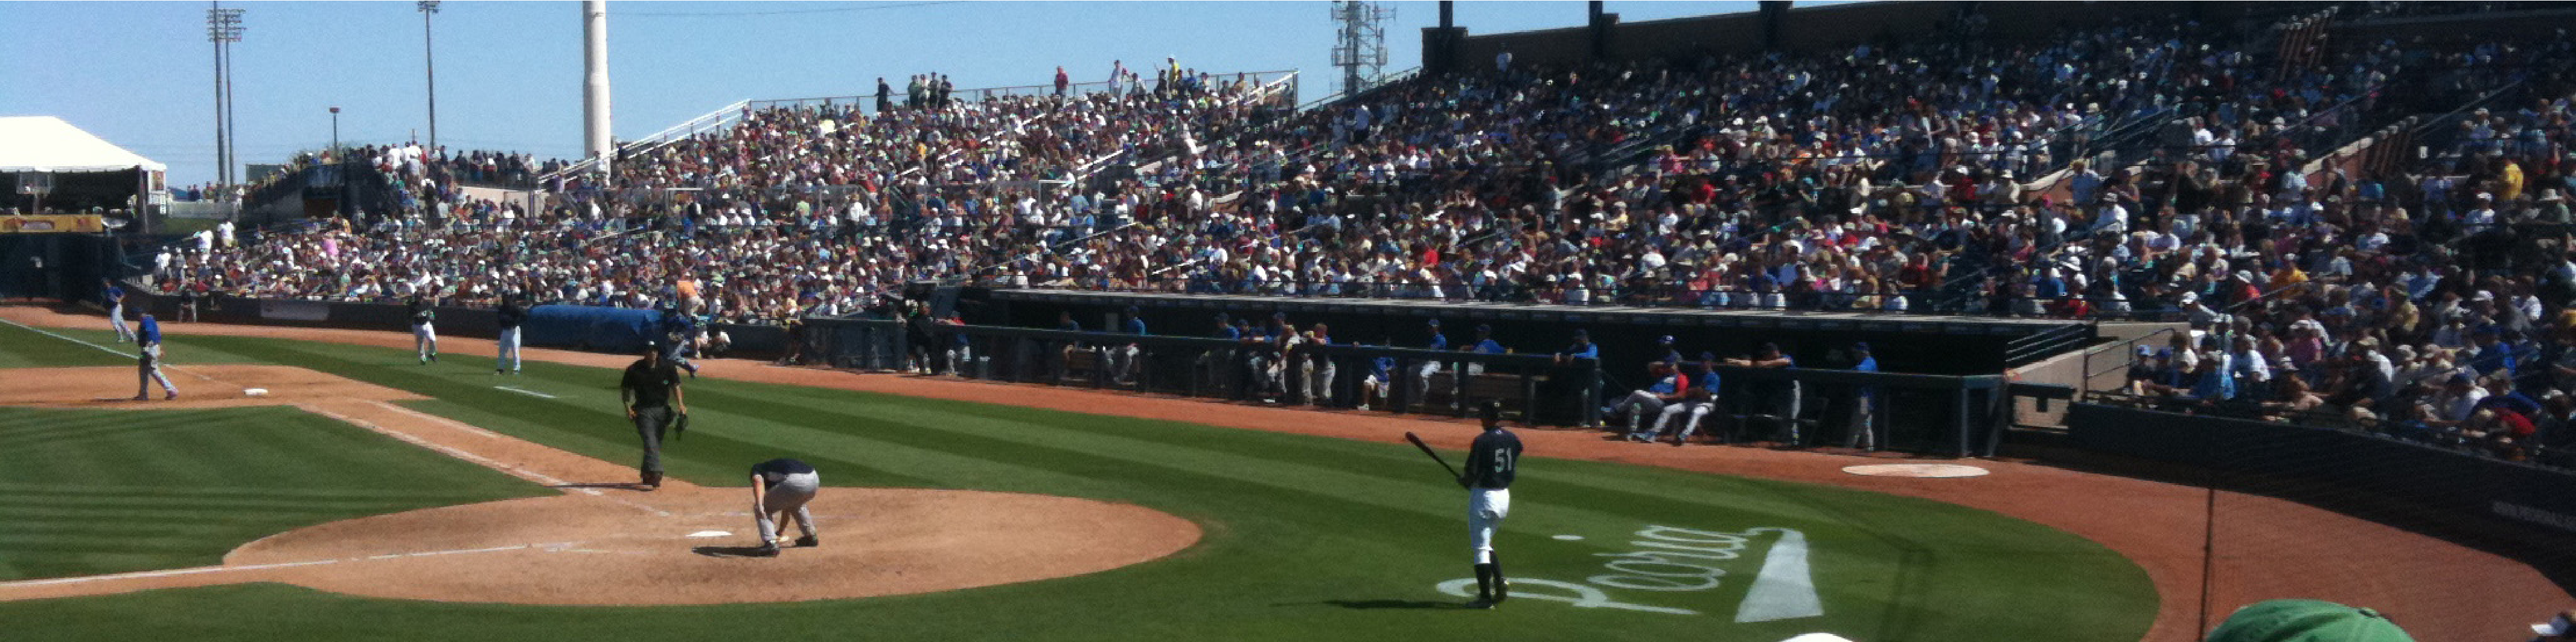
\includegraphics[width=\textwidth]{sampleteaser}
    \caption{figure caption}
    \Description{figure description}
  \end{teaserfigure}
\end{verbatim}

\section{Citations and Bibliographies}

The use of \BibTeX\ for the preparation and formatting of one's
references is strongly recommended. Authors' names should be complete
--- use full first names (``Donald E. Knuth'') not initials
(``D. E. Knuth'') --- and the salient identifying features of a
reference should be included: title, year, volume, number, pages,
article DOI, etc.

The bibliography is included in your source document with these two
commands, placed just before the \verb|\end{document}| command:
\begin{verbatim}
  \bibliographystyle{ACM-Reference-Format}
  \bibliography{bibfile}
\end{verbatim}
where ``\verb|bibfile|'' is the name, without the ``\verb|.bib|''
suffix, of the \BibTeX\ file.

Citations and references are numbered by default. A small number of
ACM publications have citations and references formatted in the
``author year'' style; for these exceptions, please include this
command in the {\bfseries preamble} (before the command
``\verb|\begin{document}|'') of your \LaTeX\ source:
\begin{verbatim}
  \citestyle{acmauthoryear}
\end{verbatim}

  Some examples.  A paginated journal article \cite{Abril07}, an
  enumerated journal article \cite{Cohen07}, a reference to an entire
  issue \cite{JCohen96}, a monograph (whole book) \cite{Kosiur01}, a
  monograph/whole book in a series (see 2a in spec. document)
  \cite{Harel79}, a divisible-book such as an anthology or compilation
  \cite{Editor00} followed by the same example, however we only output
  the series if the volume number is given \cite{Editor00a} (so
  Editor00a's series should NOT be present since it has no vol. no.),
  a chapter in a divisible book \cite{Spector90}, a chapter in a
  divisible book in a series \cite{Douglass98}, a multi-volume work as
  book \cite{Knuth97}, a couple of articles in a proceedings (of a
  conference, symposium, workshop for example) (paginated proceedings
  article) \cite{Andler79, Hagerup1993}, a proceedings article with
  all possible elements \cite{Smith10}, an example of an enumerated
  proceedings article \cite{VanGundy07}, an informally published work
  \cite{Harel78}, a couple of preprints \cite{Bornmann2019,
    AnzarootPBM14}, a doctoral dissertation \cite{Clarkson85}, a
  master's thesis: \cite{anisi03}, an online document / world wide web
  resource \cite{Thornburg01, Ablamowicz07, Poker06}, a video game
  (Case 1) \cite{Obama08} and (Case 2) \cite{Novak03} and \cite{Lee05}
  and (Case 3) a patent \cite{JoeScientist001}, work accepted for
  publication \cite{rous08}, 'YYYYb'-test for prolific author
  \cite{SaeediMEJ10} and \cite{SaeediJETC10}. Other cites might
  contain 'duplicate' DOI and URLs (some SIAM articles)
  \cite{Kirschmer:2010:AEI:1958016.1958018}. Boris / Barbara Beeton:
  multi-volume works as books \cite{MR781536} and \cite{MR781537}. A
  couple of citations with DOIs:
  \cite{2004:ITE:1009386.1010128,Kirschmer:2010:AEI:1958016.1958018}. Online
  citations: \cite{TUGInstmem, Thornburg01, CTANacmart}. Artifacts:
  \cite{R} and \cite{UMassCitations}.

\section{Acknowledgments}

Identification of funding sources and other support, and thanks to
individuals and groups that assisted in the research and the
preparation of the work should be included in an acknowledgment
section, which is placed just before the reference section in your
document.

This section has a special environment:
\begin{verbatim}
  \begin{acks}
  ...
  \end{acks}
\end{verbatim}
so that the information contained therein can be more easily collected
during the article metadata extraction phase, and to ensure
consistency in the spelling of the section heading.

Authors should not prepare this section as a numbered or unnumbered {\verb|\section|}; please use the ``{\verb|acks|}'' environment.

\section{Appendices}

If your work needs an appendix, add it before the
``\verb|\end{document}|'' command at the conclusion of your source
document.

Start the appendix with the ``\verb|appendix|'' command:
\begin{verbatim}
  \appendix
\end{verbatim}
and note that in the appendix, sections are lettered, not
numbered. This document has two appendices, demonstrating the section
and subsection identification method.

\section{Multi-language papers}

Papers may be written in languages other than English or include
titles, subtitles, keywords and abstracts in different languages (as a
rule, a paper in a language other than English should include an
English title and an English abstract).  Use \verb|language=...| for
every language used in the paper.  The last language indicated is the
main language of the paper.  For example, a French paper with
additional titles and abstracts in English and German may start with
the following command
\begin{verbatim}
\documentclass[sigconf, language=english, language=german,
               language=french]{acmart}
\end{verbatim}

The title, subtitle, keywords and abstract will be typeset in the main
language of the paper.  The commands \verb|\translatedXXX|, \verb|XXX|
begin title, subtitle and keywords, can be used to set these elements
in the other languages.  The environment \verb|translatedabstract| is
used to set the translation of the abstract.  These commands and
environment have a mandatory first argument: the language of the
second argument.  See \verb|sample-sigconf-i13n.tex| file for examples
of their usage.

\section{SIGCHI Extended Abstracts}

The ``\verb|sigchi-a|'' template style (available only in \LaTeX\ and
not in Word) produces a landscape-orientation formatted article, with
a wide left margin. Three environments are available for use with the
``\verb|sigchi-a|'' template style, and produce formatted output in
the margin:
\begin{itemize}
\item {\verb|sidebar|}:  Place formatted text in the margin.
\item {\verb|marginfigure|}: Place a figure in the margin.
\item {\verb|margintable|}: Place a table in the margin.
\end{itemize}

%%
%% The acknowledgments section is defined using the "acks" environment
%% (and NOT an unnumbered section). This ensures the proper
%% identification of the section in the article metadata, and the
%% consistent spelling of the heading.
\begin{acks}
To Robert, for the bagels and explaining CMYK and color spaces.
\end{acks}

%%
%% The next two lines define the bibliography style to be used, and
%% the bibliography file.
\bibliographystyle{ACM-Reference-Format}
\bibliography{sample-base}

%%
%% If your work has an appendix, this is the place to put it.
\appendix

\section{Research Methods}

\subsection{Part One}

Lorem ipsum dolor sit amet, consectetur adipiscing elit. Morbi
malesuada, quam in pulvinar varius, metus nunc fermentum urna, id
sollicitudin purus odio sit amet enim. Aliquam ullamcorper eu ipsum
vel mollis. Curabitur quis dictum nisl. Phasellus vel semper risus, et
lacinia dolor. Integer ultricies commodo sem nec semper.

\subsection{Part Two}

Etiam commodo feugiat nisl pulvinar pellentesque. Etiam auctor sodales
ligula, non varius nibh pulvinar semper. Suspendisse nec lectus non
ipsum convallis congue hendrerit vitae sapien. Donec at laoreet
eros. Vivamus non purus placerat, scelerisque diam eu, cursus
ante. Etiam aliquam tortor auctor efficitur mattis.

\section{Online Resources}

Nam id fermentum dui. Suspendisse sagittis tortor a nulla mollis, in
pulvinar ex pretium. Sed interdum orci quis metus euismod, et sagittis
enim maximus. Vestibulum gravida massa ut felis suscipit
congue. Quisque mattis elit a risus ultrices commodo venenatis eget
dui. Etiam sagittis eleifend elementum.

Nam interdum magna at lectus dignissim, ac dignissim lorem
rhoncus. Maecenas eu arcu ac neque placerat aliquam. Nunc pulvinar
massa et mattis lacinia.

\end{document}
\endinput
%%
%% End of file `sample-authordraft.tex'.
